
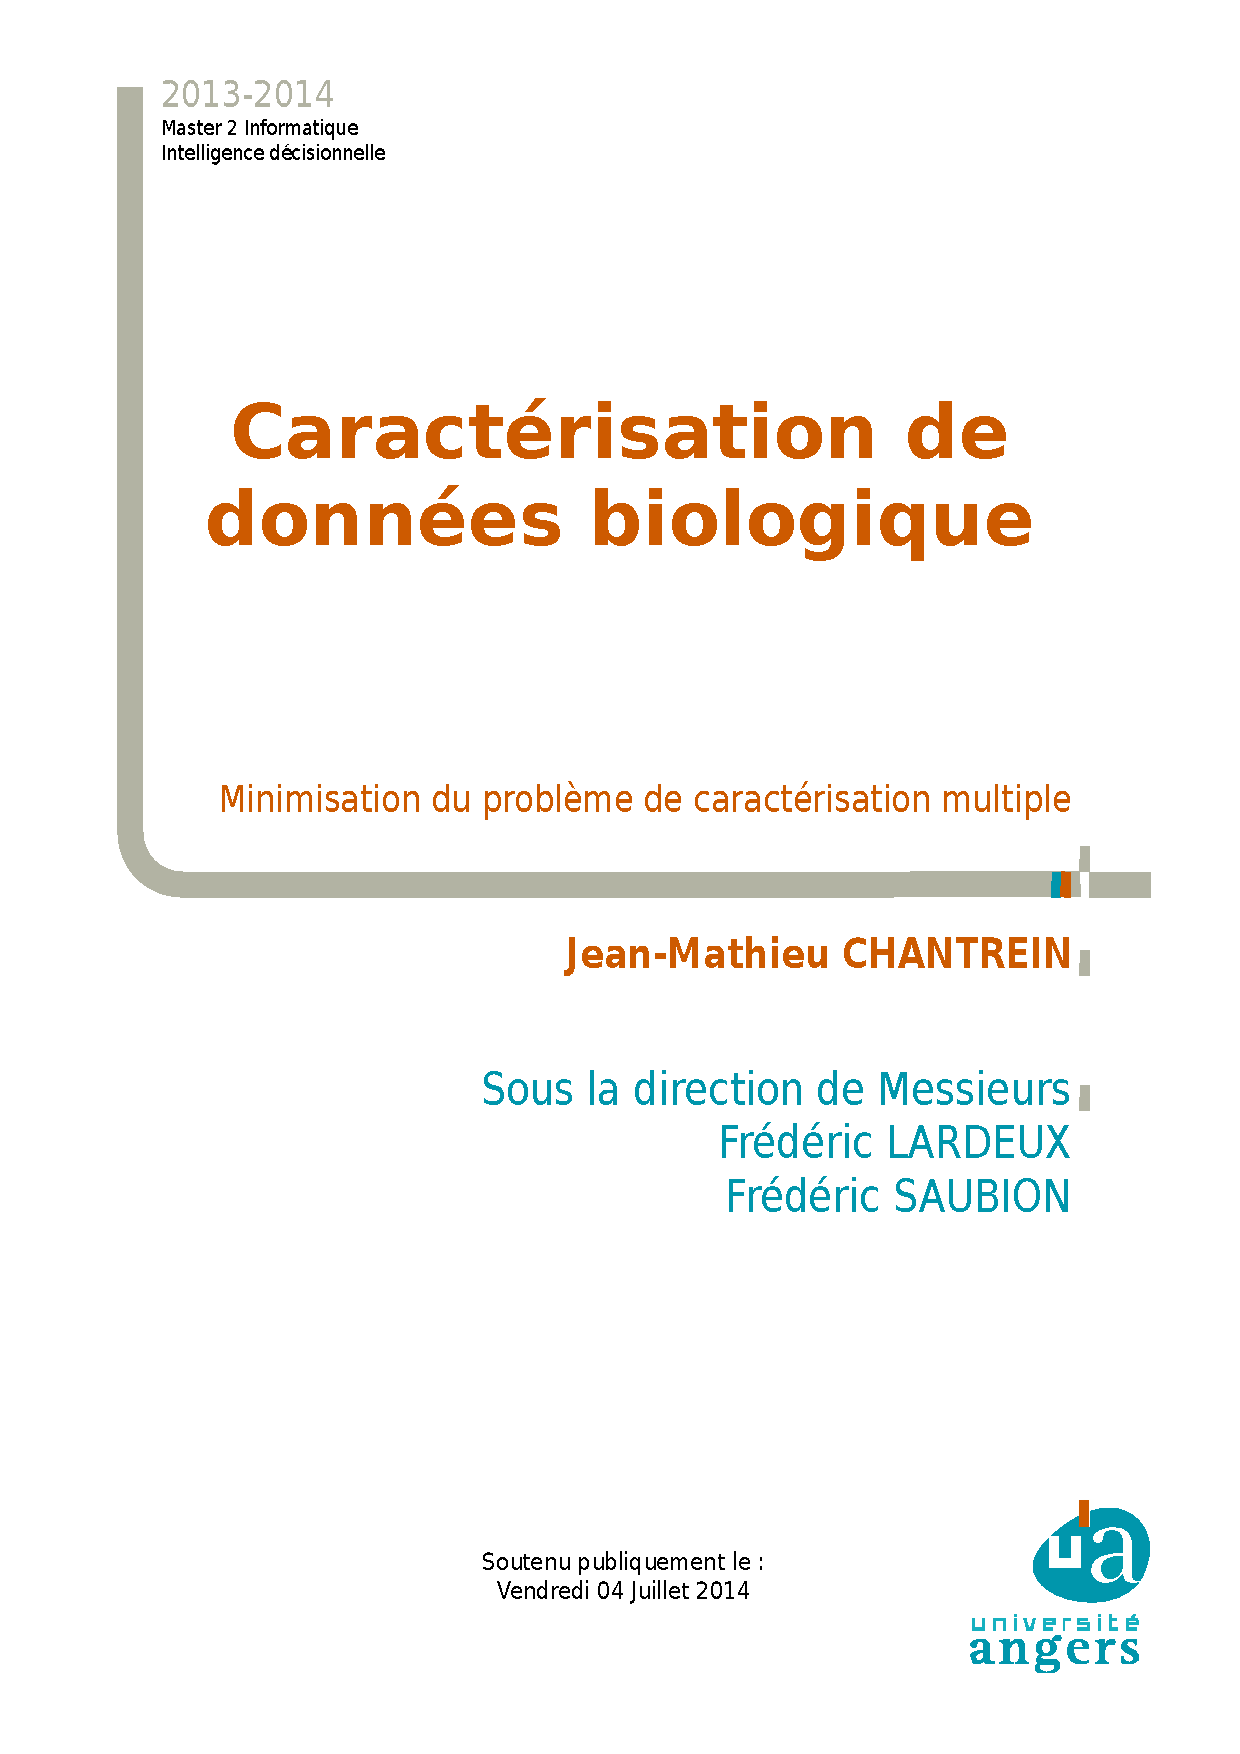
\includepdf[pages=1]{couverture/couverture.pdf}

\includepdf[pages=1]{couverture/nonPlagiat.pdf}
%
%\section*{\begin{center}Remerciements\end{center}}
%\par Tout d'abord, je tiens à remercier Frédéric LARDEUX et Frédéric SAUBION pour leur écoute, leurs disponibilités et leurs explications et pour la liberté qu'ils m'ont laissé lors de la réalisation de ce projet.
%\par Je remercie également les membres du LERIA\footnote{Laboratoire d'études et de recherche en informatique d'Angers}, pour m'avoir accordé leur confiance en m'attribuant ce stage.
%\par Je remercie l'équipe enseignante du DAEU\footnote{Diplôme d'accès aux études universitaire} d'Angers, et particulièrement Eric SCHRAFSTETTER qui m'a mis le pied à l'étrier pour intégrer la faculté des sciences d'Angers.
%\par Enfin, je remercie ma famille, qui m'a toujours soutenu dans la reprise de mes études, et tout particulièrement Lucie, Marius et Paulin qui partagent mes humeurs et mon quotidien.
%
%
%\newpage
%\null
%\begin{flushright}
%\vspace{\fill}
%\textbf{À Marius et Paulin.}
%\vspace{\fill}
%\end{flushright}


\section*{Introduction}
\subsection*{Sujet du stage}
\par La plupart des bactéries appartenant au genre Xanthomonas sont responsables de pathologies sur
une large gamme de cultures économiquement importantes, induisant notamment des pertes
de rendement et diminuant ainsi la valeur marchande des semences. Quelques graines
contaminées suffisent à générer une source d'inoculation primaire et à occasionner ainsi une
dissémination ultérieure plus large. En particulier, le pathovar phaseoli de Xanthomonas axonopodis
(Xap) qui regroupe toutes les souches identifiées comme pathogènes sur le haricot n'est pas
endémique en Europe mais pour limiter son introduction, il est inscrit sur la liste des agents
pathogènes de quarantaine. Une approche possible pour l'identification des souches bactériennes
consiste à utiliser un répertoire de gènes de virulence. Il s'agit ainsi de trouver la plus petite
combinaison de gènes de virulence spécifiques. Cette combinaison peut ainsi être utilisée pour
concevoir un test d'identification. Des travaux préliminaires[CHHEL et al.2013] montrent que la combinaison des
tests moléculaires ainsi obtenus fournit une technique rapide pour l'identification de toutes les
souches de Xanthomonas pathogènes sur les haricots.
\par Avec les possibilités accrues d'acquisition de données génomiques – par exemple le séquençage à
haut débit – mais également phénotypiques, le problème de la caractérisation de données
biologiques devrait rapidement devenir l'un des verrous essentiel de l'exploitation effective des
grandes bases de données qui sont en cours de constitution, et constituera donc un centre d'intérêt
commun aux biologistes des domaines du végétal ou de la santé. La caractérisation telle que nous
l'entendons permet d'identifier les caractères propres, éventuellement hétérogènes, d'un groupe
d’individus partageant des spécificités fonctionnelles communes (par exemple pathologiques).
\par Du point de vue informatique, ce problème est abordé comme la recherche d'un ensemble de
formules propositionnelles (variables booléennes) permettant de caractériser de manière exacte les
groupes de pathogènes. Les algorithmes mis en jeu reposent sur des explorations arborescentes
(Branch \& Bound) et des algorithmes heuristiques (recherche locale).
\par L'objectif de ce stage est double :
\begin{itemize}
\item D'une part il s'agit de constituer de nouveaux jeux de données, en dialogue avec nos collègues
biologistes. Ceci requiert la définition de formats et l'exploration de base de données pour la collecte
d'informations pertinentes. Ce travail sera effectué en lien étroit avec les laboratoires de l'INRA
Angers.
\item D'autre part, il s'agit également d'améliorer les algorithmes existants et de proposer de nouvelles
approches pour traiter des instances de grande taille. Cette phase s'inspire des algorithmes de
résolution de problèmes combinatoires (SAT-CSP).
\end{itemize}

\subsection*{Plan du rapport}
Dans la première partie de ce mémoire, nous dressons un état de l'art concernant l'étude du MIN-PCM. Celui-ci reprend les grands axes présentés dans l'article \cite{Chhel2013}. Ensuite nous décrivons les contributions que nous apportons à l'étude de ce problème: nous définissons la notion d'instance difficile, nous proposons des heuristiques de résolution (exactes ou approchées) et nous fournissons les résultats ainsi obtenus. Enfin, nous tirons les conclusions de nos travaux et nous discutons les perspectives de recherche envisagées.

% La table des matières
\newpage
\setcounter{tocdepth}{3}
\tableofcontents
\newpage

\section{État de l'art}

%\subsection{Notations}
%Dans ce mémoire, nous utilisons les notations suivantes:
%\begin{itemize}
%\item $\mathcal{X}$ représente l'ensemble des gènes d'une instance non redondante.
%\item $\mathcal{G}$ représente l'ensemble des gènes d'une instance non redondante.
%\item $\mathcal{E}$ représente l'ensemble des gènes d'une instance non redondante.
%\item $|\mathcal{X}|$ représente la cardinalité de l'ensemble $\mathcal{X}$.
%\item $|\mathcal{G}|$ représente la cardinalité l'ensemble $\mathcal{G}$.
%\item $|\mathcal{E}|$ représente la cardinalité l'ensemble $\mathcal{E}$.
%\end{itemize}




\subsection{Présentation du problème}
La plupart des bactéries appartenant au genre Xanthomonas sont responsables de pathologies sur une large gamme de cultures économiquement importantes,  induisant notamment  des pertes de rendement et diminuant ainsi la valeur marchande des semences. Quelques graines contaminées sont suffisantes pour générer une source d'inoculation primaire et occasionner ainsi une dissémination ultérieure plus large. En particulier, le pathovar\footnote{La notion de pathovar correspond à une subdivision du genre ayant des caractéristiques pathologiques observées communes.} phaseoli de  Xanthomonas Axonopodis (Xap) qui regroupe toutes les souches identifiées comme pathogènes sur le haricot \cite{Vauterin1995}, n'est pas endémique en Europe mais pour limiter son introduction, il est inscrit sur la liste des agents pathogènes de quarantaine.

La taxonomie du genre Xanthomonas n'est pas encore pleinement résolue, et la délimitation de certaines espèces dans ce genre fait encore débat \cite{Schaad2005}~; les approches phylogénétiques ne sont alors pas réellement applicables. Une approche possible pour l'identification des souches bactériennes consiste à utiliser un répertoire de gènes de virulence. Il s'agit ainsi de trouver la plus petite combinaison de gènes de virulence spécifiques au Xap. Cette combinaison peut être utilisée pour concevoir un test PCR multiplex pour l'identification de Xap \cite{Boureau2013,Boureau2012} dont le coût est directement lié au nombre de gènes à tester. Les résultats obtenus
montrent que la combinaison des tests moléculaires ainsi obtenus fournit une technique rapide pour l'identification de toutes les souches de Xanthomonas pathogènes sur les haricots.

Plus formellement, considérons un ensemble d'entités (les souches bactériennes) regroupées en groupes (les pathovars). Chaque entité est définie par la présence ou l'absence d'un ensemble de caractères (les gènes). Au regard de la représentation binaire qui est utilisée, une entité est considérée comme une interprétation booléenne sur les caractères, qui seront donc les variables booléennes du problème. Ainsi, pour chaque groupe, l'ensemble des entités fournit une table de vérité partielle d'une fonction booléenne vraie pour les interprétations correspondant aux entités du groupe et fausse pour toutes les autres entités des autres groupes. Une telle fonction sera appelée caractérisation d'un groupe. Ces fonctions booléennes seront représentées par des formules propositionnelles construites sur un langage fixé.



Le problème de caractérisation multiple consiste ainsi à trouver un ensemble de
formules booléennes de sorte que chaque formule soit une caractérisation. Le terme
multiple désigne le fait qu'il faut considéroer un ensemble de groupes dont les
caractérisations sont dépendantes des entités contenues dans ceux-ci mais aussi
des entités appartenant aux autres groupes.

\begin{figure}[H]{Exemple de problème de caractérisation multiple}
\begin{center}
\begin{tabular}{|c||c|c|c|c|}
\hline
\multirow{2}{*}{Souches}&\multirow{2}{*}{Groupes}&\multicolumn{3}{c|}{Caractères
}\\
&&$a$&$b$&$c$\\
\hline
\hline
$e_1$&\multirow{2}{*}{$g_1$}&\cellcolor{lightgray}0&\cellcolor{lightgray}0&0\\
\cline{1-1} \cline{3-5}
$e_2$&&\cellcolor{lightgray}0& \cellcolor{lightgray}0&1\\
\hline
\hline
$e_3$&$g_2$&1&\cellcolor{lightgray}1&\cellcolor{lightgray}1\\
\hline
\hline
$e_4$&\multirow{2}{*}{$g_3$}&1&\cellcolor{lightgray}1&\cellcolor{lightgray}0\\
\cline{1-1} \cline{3-5}
$e_5$&&0&\cellcolor{lightgray}1&\cellcolor{lightgray}0\\
\hline
\end{tabular}
\end{center}
\caption{}
\label{CD}
\end{figure}

Dans la figure  il y a 5 entités réparties dans 3 groupes et dont
la description se base sur un ensemble de 4 caractères.
Résoudre ce problème revient à caractériser chaque groupe. Il faut donc, pour
chaque groupe, trouver une combinaison de  variables permettant de construire une formule vraie pour toutes les
entités du groupe et fausse pour les autres entités des autres
groupes. Dans l'exemple de la figure \ref{CD}, le groupe 1 est caractérisé par
la négation des variables $a$ et $b$  alors que le groupe 2 est caractérisé par
les variables $b$ et $c$. Les souches du groupe 3 ont toutes en commun la
négation de la variable $c$ tout comme l'entité $e_1$ du groupe 1. Il faut donc
ajouter une autre variable ($b$ par exemple) pour être sûr de caractériser le
groupe.
\subsection{Problème de caractérisation multiple}
Nous présentons dans cette section le problème de caractérisation multiple ainsi que les diverses méthodes qui ont été proposés dans \cite{Chhel2012,Chhel2013} et qui permettent de résoudre le MIN-PCM.

\subsubsection{Présentation du problème}

\begin{definition}[Instance du PCM]
Une instance du problème de caractérisation multiple est définie par un n-uplet
$({\cal X}, {\cal E}, {\cal G})$ où $\cal X$ est l'ensemble des
variables propositionnelles, ${\cal E}$ est l'ensemble des entités définies sur
$\cal X$ et ${\cal G} \subseteq 2^{\cal E}$.
\end{definition}

Chaque entité représente une affectation booléenne, ou interprétation, définit ainsi  $e : {\cal X} \to \{0,1\}$, où  $0$ et $1$ sont respectivement les valeurs de vérité fausse et vraie. $e(x)$ correspond donc à la valeur de vérité affectée à $x$ dans l'interprétation $e$. Pour une formule propositionnelle  $\phi$ quelconque sur ${\cal X}$, nous notons $e \models \phi $ le fait que l'interprétation $e \in {\cal E}$ satisfait la formule $\phi$. Une entité $e \in {\cal E}$ sera classiquement représentée par un n-uplet de valeur booléennes (un élément de  $ \{0,1\}^n$).   Ainsi, une instance $({\cal X}, {\cal E}, {\cal G})$  peut être vue comme une matrice booléenne dont les $n$ colonnes correspondent aux variables booléennes de ${\cal X}$ et les $m$ lignes aux entités de ${\cal E}$.  Chaque variable $x_j$ correspond à la colonne $j \in \{1, \ldots, n \} $. Chaque entité $e_i$ correspond à une ligne $i \in \{1, \ldots, m \}$.

Nous pouvons appliquer des prétraitements pour réduire la taille de la matrice en réduisant le nombre de variables réellement utiles et/ou le nombre d'entités. Nous définissons ainsi la notion d'instance non redondante.

\begin{definition}[Instance non redondante]
Une instance est non redondante ssi :
\begin{itemize}
\item Il n'existe pas de colonnes dont toutes valeurs sont identiques :

$\nexists j \in \{1,\ldots, n \},\forall i \in \{1, \ldots, m \} $ tel que $a_{ij}=1$ (resp $a_{ij}=0$);
\item Chaque colonne est unique :

$\nexists j \in \{1, \ldots, n \},\forall k \in \{1, \ldots, n \} \setminus \{j\}, \forall i \in \{1, \ldots, m \} $ tel que $a_{ij}=a_{ik}$;
\item Chaque entité est unique : \\$ \nexists i \in \{1, \ldots, m \},
\forall l \in \{1, \ldots, m \} \setminus \{i\},\forall j \in \{1, \ldots, n \},$ tel que $e_i(x_j)=e_l(x_j)$.
\end{itemize}
\end{definition}

L'application d'un algorithme d'élimination de la redondance s'effectue au pire des cas en ${\mathcal O}({|\cal X}|^2+|{\cal E}|^2)$ et peut conduire à une instance mal-formée dont toutes les colonnes ont été supprimées ou possédant des groupes vides.

Une fois l'instance réduite, nous pouvons préciser la notion de solution d'un problème de caractérisation multiple.

\begin{definition}[Caractérisation d'un groupe]
Pour une instance $({\cal X}, {\cal E}, {\cal G})$, une formule $\phi_g$
caractérise un groupe $g\in {\cal G}$ ssi :
$\forall e \in g, e \models \phi_g$ (acceptation des entités du groupe) et
$\forall g' \in {\cal G} \setminus \{g\},\forall e' \in g',  e' \not \models
\phi_g$ (rejet des entités des autres groupes).
\end{definition}

Par extension, nous notons $g \models \phi_g$ le fait que $\phi_g$ caractérise $g$ selon la définition précédente. $Sol(g)$ représente l'ensemble des solutions d'un groupe $g$. $Sol(g)=\{\phi_g|g \models \phi_g\}$.

\begin{definition}[Solution d'un PCM ]
Pour une instance $({\cal X}, {\cal E}, {\cal G})$, une solution
admissible du PCM  est un $|{\cal G}|$-uplet de formules
$\Phi=(\phi_1,\cdots,\phi_{{\cal G}})$ tel que  $\forall i\in \{1,\ldots,|G|\}, g_i \in
{\cal G}$, $g_i \models \phi_i$.
\end{definition}

Soit ${\cal I} = ({\cal X}, {\cal E}, {\cal G})$, $ SOL({\cal I})$ est
l'ensemble de toutes les solutions multiples pour tous les groupes. $SOL({\cal
I})=Sol(g_1) \times \cdots \times Sol(g_{|{\cal G}|})$, où $\times$ désigne le produit cartésien. Pour un ensemble de
groupes ${\cal G}$ et un $|G|$-uplet de formules $\Phi=(\phi_1,\cdots,\phi_{|{\cal G}|})$, nous notons par extension ${\cal G} \models \Phi$ le fait que
$\forall i\in \{1,\ldots,|G|\}, g_i \in {\cal G}$, $g_i \models \phi_i$.

\begin{definition}[Satisfiabilité d'un PCM]
Une instance $({\cal X}, {\cal E}, {\cal G})$ est satisfiable (resp. insatisfiable) ssi
$\forall g \in {\cal G}, Sol(g) \neq \emptyset$ (resp. $\exists g \in {\cal G},
Sol(g) = \emptyset$).
\end{definition}

Il est évident que toute instance possédant deux interprétations identiques dans deux groupes différents n'est pas satisfiable d'où :

\begin{proposition}
Une instance $({\cal X},{\cal E},{\cal G})$ est satisfiable $\Leftrightarrow
\forall g,g' \in {\cal G}, g\neq g', g
\cap g' =\emptyset$.
\end{proposition}

Une conséquence immédiate est qu'une instance non redondante et bien formée
est satisfiable puisque chaque entité a une interprétation unique.
En pratique, le test de satisfiabilité est effectué implicitement lors de
l'étape de prétraitement et à charge de l'utilisateur de modifier ou supprimer
les entités mis en cause dans l'échec de ce test.

\begin{definition}[Taille d'un n-uplet de formule]
\label{Flength}
Pour un n-uplet $\Phi=(\phi_1,\cdots,\phi_n)$ nous avons $|\Phi| =
|\bigcup_{\phi_i} var(\phi_{i})|$, où $var({\phi})$ retourne l'ensemble des
variables de
$\phi$.
\end{definition}

\begin{definition}[k-PCM (problème de décision)]
Soit une instance ${\cal I}$ une
caractérisation multiple minimale $k$ est un ensemble de formules
$\Phi \in Sol({\cal I})$ vérifiant $|\Phi| \leq k$ avec $ k\in \mathbb{N}^{+}$.
\end{definition}

Le problème de caractérisation multiple minimale pour une taille $k$ ne
correspond pas nécessairement à une solution minimale de
$(\phi_1,\cdots,\phi_n)$ telle que chaque $\phi_i$ est un élément minimal de
$Sol(g_i)$. Nous définissons le problème d'optimisation comme suit.

\begin{definition}[MIN-PCM (problème d'optimisation)]
Pour une instance ${\cal I}$, une
caractérisation optimale multiple minimale est  un ensemble de formules
$\Phi^* \in Sol({\cal I})$ vérifiant $|\Phi^*| \leq |\Phi|$ avec $\forall \Phi
\in Sol({\cal I})$
\end{definition}

\subsubsection*{Minimisation du problème de caractérisation multiple}
La minimisation du problème de caractérisation multiple consiste à définir le plus petit nombre de gène pouvant caractériser une instance PCM.


\subsection{Complexité}
Le problème SET-COVER appartient à la classe de complexité W[2]-complet. Il a été montré dans \cite{Chhel2013} qu'une instance PCM pouvait être réduite en temps polynômial en une instance SET-COVER. Il en résulte que PCM appartient à la classe de complexité W[2]-complet \footnote{En admettant l'hypothèse que la WEFT-hiérarchie proposé par [Downey, Fellows, 1995] soit correcte.}. Dès lors, il a été prouvé que le MIN-PCM appartient à la classe de complexité W[2]-difficile. L'impact direct de l'appartenance de MIN-PCM à cette classe de complexité est que l'\textbf{unique} possibilité d'améliorier significativement la résolution complète\footnote{Recherche exacte permettant de prouver l'optimalité d'une solution.} d'une instance est de \textbf{travailler sur des heuristiques de choix de variables}(gènes). 

\subsection{Méthode de résolution}
Toutes les méthodes présentées dans cette sous-section sont issus de \cite{Chhel2013}.

\subsubsection{Une résolution basés sur les fonctions booléenes partiellement définis}

Les fonctions booléennes partiellement définies, {\em partially
defined Boolean formula - pdBf},  \cite{Iba99} permettent de proposer un
cadre de résolution intéressant.

Une pdBf est vue comme une fonction booléenne pour laquelle  certaines interprétations ne
sont pas définies.
La classe ${C}^{+}$ (resp. ${C}^{-}$)  désigne l'ensemble des exemples positifs
(resp. négatifs).
À partir de toute fonction booléenne, nous pouvons calculer une formule
caractérisant l'ensemble des interprétations, appelée extension. Il en est de
même pour les pdBf où une DNF (formule en forme normale disjonctive) est une
extension facilement calculable caractérisant la classe $\mathcal{C}^+$.

En ce qui concerne le PCM, nous construisons un ensemble de pdBf emboîtées où
chaque classe ${C}^{-}$ est l'union des classes ${C}^{+}$ des autres groupes.
Nous nous appuyons sur la notion de projection pour calculer de nouvelles
solutions.

\begin{definition}[Projection]
Une projection $\pi$ d'une instance ${\cal I}$ de PCM est la donnée d'un
sous-ensemble ${\cal X'} \subseteq {\cal X}$, définissant implicitement
l'instance ${\cal I'} = ({\cal X'},\{\pi(e) \mid e \in  {\cal E} \},\{ \pi(g)
\mid g \in {\cal G}\})$, où $\pi(e)$ est la restriction de $e$ aux variables de
${\cal X'}$, et $\pi(g)$ est $\{\pi(e)\mid e\in g\}$. On appelle
\emph{dimension} d'une projection $\pi$  le cardinal de ${\cal X'}$.
\end{definition}

La minimisation du nombre de colonnes pour le problème PCM revient à chercher la
projection satisfiable de plus petite dimension associée aux pdBf de chaque
groupe.

La principale difficulté du PCM ne dépend pas de la structure des formules de
l'ensemble solution mais du choix des variables présentes dans celui-ci. La
satisfiabilité d'un ensemble de formules de taille $k$  pour une instance du PCM est équivalente au fait que nous cherchons un sous-ensemble de pdBf consistantes, issues d'une projection satisfiable de dimension $k$ sur les pdBf initiales.

%\subsection{Application : test de diagnostic en biologie végétale}
%
%Nous présentons dans cette section l'utilisation du PCM dans le contexte de la biologie végétale.
%
%\subsubsection{La caractérisation de pathovars}
%
%Comme mentionné en introduction, la bactérie {\em Xanthomonas}  cause de gros
%dégâts sur certaines cultures. Les différentes souches de cette bactérie sont
%réparties en groupes et leurs caractéristiques (génotypiques ou phénotypiques)
%sont connues. L'objectif est de créer un test de diagnostic permettant de
%détecter rapidement à quel groupe appartient une souche donnée.
%
%La caractérisation précise des collections de souches bactériennes est un enjeu
%scientifique majeur, car ces bactéries sont responsables d'importantes
%pathologies végétales, et donc soumises à des procédures de contrôles officiels
%(par exemple, en Europe, la directive 2000/29/CE). Le développement de tests de
%diagnostic est donc crucial pour identifier systématiquement les
%souches de ces espèces. Dans ce contexte, le problème de caractérisation
%correspond à l'identification d'un groupe de souches vis-à-vis d'autres groupes,
%basée sur la présence ou l'absence de certains caractères particuliers
%\cite{plos}. Une souche peut donc être vue comme un vecteur de valeurs binaires
%qui reflète la présence (valeur 1) ou l'absence (valeur 0) de ces caractères. De
%plus, les tests de diagnostic étant basés sur des puces à ADN, il est nécessaire
%de chercher à minimiser les solutions (le nombre de tests associés pour chaque
%identification) afin de réduire le coût prohibitif de ces tests. Notons également que pour chaque caractère le spot de test doit être dupliqué sur la puce, ce qui réduit d'autant plus le nombre de caractères utilisables pour un même kit de diagnostic. Ce problème correspond exactement au MIN-PCM.

\subsubsection{Résolutions complètes}
\paragraph{\emph{Exact-Proj-Car}}
Le solveur \emph{Exact-Proj-Car}, proposé dans \cite{sac12}, est basé sur une approche complète consistant à valider ou non la présence d'une caractérisation de taille $k$. Deux types d'exploration sont possibles :
\begin{itemize}
 \item Une exploration en largeur consistant à montrer qu'il n'existe aucune caractérisation valide de taille $k$ avant de tester celles de taille $k+1$. En commençant avec $k= \lceil
log_2(|\cal{G}|)\rceil$ il est donc garanti de trouver la caractérisation valide optimale. En effet, il est impossible de distinguer plus de $2^k$ classes avec une projection de dimension $k$.
 \item Une exploration en profondeur partant de la caractérisation maximale (toutes les variables) et recherchant une caractérisation valide de taille $k-1$ dès qu'une caractérisation valide de taille $k$ est trouvée.
\end{itemize}

Ces deux approches garantissent toutes les deux de trouver une caractérisation valide optimale mais en cas d'arrêt de la recherche (temps limite atteint, ...), seule l'exploration en profondeur est capable de fournir une caractérisation valide. De plus, en termes de nombre de caractérisations testées, l'exploration en largeur semble la plus coûteuse (hormis pour les solutions de très petite taille). En effet, il est évident que l'exploration en largeur traitera au moins $\binom{n}{k}$ caractérisations ($n$ étant le nombre de variables totales) alors que pour l'exploration en profondeur il est impossible de prévoir ce nombre (au mieux $n-k$ et au pire $\sum_{i=n}^{i=k}\binom{n}{i}$). Remarquons que l'utilisation conjointe de ces deux méthodes permet de borner la caractérisation optimale.

Ces explorations ont toutes les deux des choix de variables à faire: une heuristique de branchement basée sur un classement des variables de manière statique au début de la recherche. L'ordre utilisé est un calcul d'entropie inspirée par la technique proposée dans \cite{DesVer81} qui privilégie les variables permettant de séparer un groupe par rapport aux autres.

\paragraph{Reformulation en programmation linéaire}

Il existe une reformulation du PCM en programmation linéaire. Nous nous intéressons plus
particulièrement à la minimisation du PCM (MIN-PCM) qui consiste à minimiser la taille  $k$ de la solution. Cette reformulation permet d'obtenir de nouveaux résultats de complexité pour le PCM.


La modélisation du
MIN-PCM peut se faire en programmation entière 0/1 (pseudo-booléen). Le MIN-PCM est reformulé sous la forme d'un problème MIN-ONES. Le problème MIN-ONES est un problème d'optimisation défini comme suit:

\begin{definition}[MIN-ONES]
Soit $ \Phi $ une collection de formules booléennes $\phi_i$ (contraintes)
définie sur  $\cal X$. Le problème consiste à trouver une affectation booléenne  sur $\cal X$ telle que
chaque contrainte soit satisfaite tout en minimisant le nombre de variable vraie dans cette affectation.
\end{definition}

Une formule booléenne est construite avec chaque paire d'entités de groupes différents.

Soit $({\cal X}, {\cal E}, {\cal G})$ une instance du PCM.
Pour toute paire d'entités $\{e_i,e_j\}\in {\cal E}^2$ telle que $e\in g,e'\in
g',g\neq g'$, nous construisons une formule $\phi$ de la manière suivante :\\
$\phi=\bigvee_{x_k \in \{x|x \in {\cal X}, e(x) \neq e'(x)\}} x_k $.

Nous observons que $\phi$ est une clause composée uniquement de littéraux positifs. L'ensemble $\Phi$ de ces formules permet de modéliser entièrement le PCM de manière à le résoudre par programmation entière 0/1.

\begin{center}
\[\begin{array}{l}
Domaine : y_i \in \{0,1\}\\
min : \sum_i y_i\\
s.t.\\
  y_{1}+\cdots+y_{n} \geq 1, \forall(x_{1}\vee\cdots\vee x_{n}) \in
\Phi\\
\end{array}\]
\end{center}

Nous constatons que la transformation d'une instance est bornée par $|{\cal E}|^2$
%\begin{exemple}[Transformation vers MIN-ONES en programmation linéaire]
%\hspace{0.1cm} 
%
%Considérons l'instance :
%\begin{center}
%\begin{tabular}{|c|c||c|c|c|c|}
%\hline
%\multirow{2}{*}{Entités}&\multirow{2}{*}{Groupes}&\multicolumn{4}{c|}{Caractères}
%\\
%&&x1&x2&x3&x4\\
%\hline
%\hline
%e1&g1&1&1&1&0\\
%\hline
%e2&g1&1&1&1&1\\
%\hline
%e3&g2&0&0&1&0\\
%\hline
%e4&g2&0&1&1&1\\
%\hline
%e5&g3&1&1&0&0\\
%\hline
%\end{tabular}
%
%\par La transformation en programmation entière 0/1 est la suivante :
%
%\[\begin{array}{l m{2cm} r}
%\multicolumn{3}{l}{min : \sum_{i=1}^{4} y_i}\\
%\multicolumn{3}{l}{s.t.} \\
%  y_1+y_2\geq 1 &&  c_{\{e1,e3\}}\\
%  y_1+y_4\geq 1&&  c_{\{e1,e4\}}\\
%  y_3 = 1&& c_{\{e1,e5\}}\\
%  y_1+y_2+y_4 \geq 1&&  c_{\{e2,e3\}}\\
%  y_1 = 1&& c_{\{e2,e4\}}\\
%  y_3 + y_4 \geq 1&&  c_{\{e2,e5\}}\\
%  y_1+y_2+y_3\geq 1&& c_{\{e3,e5\}}\\
%  y_1+y_3 + y_4 \geq 1&&  c_{\{e4,e5\}}
%\end{array}\]
%
%\end{center}
%où chaque contrainte ($c_{\{e_i,e_j\}}$) correspond au traitement d'une paire
%d'entités.
%\end{exemple}
%
%Avec la transformation proposée, nous pouvons constater qu'une même contrainte
%ne peut apparaître plusieurs fois quel que soit le nombre de groupes du départ si
%l'instance est d'une part non redondante pour les entités et d'autre part
%satisfiable. Bien évidement cela impose de construire l'ensemble des contraintes
%en imposant un ordre sur les entités.
%
%Dans \cite{creignou2001complexity}, les auteurs établissent que  MIN-ONES en
%présence de clauses ne possédant que des littéraux positifs est contenu dans la
%classe de complexité APX \cite{PapadimitriouY91}, ce qui laisse penser
%que PCM est approximable\cite{Chhel2013}.

%\subparagraph{Réduction d'une instance du problème en programmation linéaire}
%\label{sec::reduc}
%La transformation du PCM afin de le résoudre à l'aide de programmation linéaire
%produit un nombre extrêmement important de clauses. Afin de réduire ce nombre, il
%est envisageable d'utiliser la détection de subsomptions \cite{sub} comme cela
%est pour le problème SAT. Ce mécanisme peut s'appliquer à
%la simplification d'une instance en programmation entière 0/1 car la définition
%particulière des contraintes sur lesquelles nous travaillons le permet
%(clauses ne contenant que des littéraux positifs). Si
%$var(c_{\{e_i,e_j\}})$, avec $i \neq j$, désigne l'ensemble des variables de
%décisions d'une contrainte  produite par la paire d'entités $\{e_i,e_j\}$, nous
%pouvons supprimer toutes contraintes ayant un sous-ensemble de variables
%correspondant à l'ensemble de variables d'une contrainte. Plus formellement,
%nous supprimons toute contrainte $c_{\{e_i,e_j\}}$ telle que $\forall
%c_{\{e_k,e_l\}}$,avec $k \neq l$, nous avons  $var(c_{\{e_k,e_l\}})\subset
%var(c_{\{e_i,e_j\}})$. Comme pour la
%subsomption, il est facile de remarquer que n'importe quelle affectation
%validant la contrainte $c_{\{e_k,e_l\}}$ implique la validité de
%$c_{\{e_i,e_j\}}$.
%
%Dans l'exemple précédent, nous calculons une solution $y_1=1$ et $y_3=1$
%en remarquant que $c_{\{e2,e4\}}$ {resp $c_{\{e1,e5\}}$}  permet de supprimer
%$c_{\{e1,e3\}}$, $c_{\{e1,e4\}}$, $c_{\{e2,e3\}}$, $c_{\{e3,e5\}}$ et
%$c_{\{e4,e5\}}$ (resp. $c_{\{e2,e5\}}$).
%
%Toutefois, il faut remarquer qu'une subsomption n'est présente que lorsque les conditions suivantes sont vérifiées :
%\begin{itemize}
%\item deux entités $e_1$ et $e_2$ d'un même groupe possèdent $x$ variables avec la même valeur~;
%\item au moins une entité d'un autre groupe a des valeurs identiques pour les $n-x$ variables non identiques de  $e_1$ ou de $e_2$ ($n$ étant le nombre total de variables).
%\end{itemize}
%
%La probabilité de réduire une instance en programmation linéaire est donc assez faible ($\frac{1}{2^{2n}}<p<\frac{1}{2^{n}}$) mais pour des instances venant de problèmes réels les conditions de subsomption sont souvent réunies.

\subsubsection{Résolution par recherche locale }
\paragraph{\emph{LS-Proj-Car}}
Utiliser une approche complète peut s'avérer inefficace dans le cas de PCM de grande taille. Une alternative est donc de résoudre le problème à l'aide d'un algorithme de recherche locale \cite{Hoos2004}. L'optimalité des résultats n'est plus garantie mais une solution de bonne qualité est généralement trouvée assez rapidement.

Le principe de l'approche appelée \emph{LS-Proj-Car} est de parcourir l'espace des projections valides en utilisant une liste tabou \cite{Glover1997} afin de limiter les risques de cycles durant la recherche. La fonction de voisinage est définie par l'ensemble des projections ayant une variable de plus ou de moins que la projection actuelle. Le passage d'un voisin à un autre se fait à l'aide de deux opérateurs : $ajout\_var$ qui ajoute aléatoirement une variable à la projection et $supprime\_var$ qui supprime la première variable permettant d'atteindre une projection valide. La recherche commence avec la projection de dimension maximale (toutes les variables) et applique $supprime\_var$ à chaque fois que cela est possible. La liste tabou permet d'éviter d'ajouter et de supprimer une variable plusieurs fois de suite.

Afin de permettre une exploration plus large de l'espace de recherche, plusieurs redémarrages de la recherche sont effectués. Pour ne pas reparcourir les mêmes projections, un mécanisme d'apprentissage permet de garantir un début de recherche différent pour chaque relance. Son principe est de donner un poids inversement proportionnel à l'ordre de sélection lors des recherches précédentes, pour chacune des variables, afin de pouvoir initier les relances suivantes en sélectionnant des variables ayant un poids faible. Ainsi, chaque relance oriente la recherche vers des zones de l'espace de recherche non explorées.
\subsection{Résultats expérimentaux}



%Le tableau \ref{tab:results}, présente plusieurs informations sur les instances ainsi que sur leur résolution par différents algorithmes sont présentées. Les colonnes "entités", "groupes" et "caractères" donnent les propriétés des instances. La colonne "contraintes" fournit le nombre de contraintes nécessaires pour reformuler chaque instance sous forme de programme linéaire, la colonne $r$ désigne le ratio entre le nombre de contraintes et le nombre d'entités et la colonne réduction indique le nombre de contraintes après réduction ("non" si aucune). Les trois dernières colonnes fournissent les résultats obtenus (nombre de variables dans la caractérisation trouvée) pour la résolution en programmation linéaire en utilisant \emph{cplex}  \footnote{\texttt{http://www.ibm.com/software/integration/optimization/cplex-optimizer/}} sur le problème réduit("PL"), pour l'exécution d'\emph{Exact-Proj-Car} ("EPJ") et enfin pour l'application de l'algorithme de recherche locale \emph{LS-Proj-Car} ("LSPC"). 











Afin d'avoir un moyen de comparaison pour nos contributions, nous reproduisons ici les résultats fourni dans \cite{Chhel2013}\footnote{Nous nous sommes servi du code mis à disposition sur \url{http://forge.info.univ-angers.fr/~gh/Idas/Ccd/mcps/}}. Les expérimentations sont faites sur une machine composé d'un processeur Intel Core\up{tm} i7-2620M CPU à 2.70GHz (deux cœurs) avec 4 Go Ram tournant sous Linux 64-bits. L'option de compilation -Ofast est activé pour obtenir notre exécutable.
\begin{itemize}
\item Les instances réelles (raphv, raphy, rarep, rch8 et rch10) sont tirées de problèmes de caractérisation provenant de l'API BioMérieux basée sur des propriétés bio-chimiques de l'espèce Ralstonia et sur des expressions de gènes de virulences de l'espèce Xanthomonas.
\item Les instances aléatoires sont générées en deux étapes, pour un nombre de variables et de groupes fixés. Tout d'abord, chaque entité est construite de manière aléatoire. Ensuite, une certaine proportion des entités est répartie de manière équitable entre tous les groupes et les entités
restantes sont affectées une à une aléatoirement aux groupes. La proportion
d'entités affectées aléatoirement est donnée en pourcentage et est appelée
$bruit$. Une instance aléatoire est notée sous la forme : s$graine$-$bruit$.
\end{itemize}
Le temps autorisé pour chaque exécution est 10 minutes. Les résultats en gras indiquent que les solutions sont optimales.
\begin{center}
\begin{tabular}{|c|c|c|c|c|c|c|}
\hline 
Instances & Entités(SR) & Groupes & Gènes(SR) & PL & EPC(DIFF)(SH) & LSPC(DIFF) \\ 
\hline 
s301-0 & 500 & 30 & 400 & - & 13 & 14 \\ 
\hline 
s326-0 & 500 & 10 & 500 & - & 13 & 14 \\ 
\hline 
s413-30 & 500 & 20 & 600 & - & 13 & \textcolor{blue}{13} (14) \\ 
\hline 
s555-20 & 800 & 20 & 800 & - & 13 & \textcolor{blue}{13} (14) \\ 
\hline 
s625-20 & 500 & 5 & 1000 & - & 13 & \textcolor{blue}{13} (14) \\ 
\hline 
s754-10 & 600 & 10 & 200 & - & 13 & 14 \\ 
\hline 
s882-20 & 600 & 10 & 400 & - & 13 & 14 \\ 
\hline 
s2501-70 & 800 & 10 & 800 & - & \textcolor{blue}{15} (14) & 15 \\ 
\hline 
s31294-50 & 200 & 15 & 1000 & 10 & 10 & 11 \\ 
\hline 
s3836-0 & 1000 & 15 & 1000 & - & 16 & 16 \\ 
\hline 
raphv & 109 (108) & 8 & 155 (68) & \textbf{6} & \textbf{6} & 9 \\ 
\hline 
raphy & 113 (112) & 4 & 155 (70) & \textbf{6} & \textbf{6} & 8 \\ 
\hline 
rarep & 112 & 7 & 155 (72) & \textbf{12} & 95 (59) (\textcolor{blue}{39}) & 14 \\ 
\hline 
rch8 & 132 (56) & 21 & 37 (27) & \textbf{9} & \textbf{9} & 9 \\ 
\hline 
rch10 & 173 (112) & 27 & 98 (86) & \textbf{10} & 27 (15) (\textcolor{blue}{25}) & 15 \\ 
\hline 
\end{tabular} 
\end{center}
Colonne PL: Résultats obtenu par reformulation en programmation linéaire sur le solveur IBM \textit{cplex}\footnote{\url{http://www.ibm.com/software/integration/optimization/cplex-optimizer}}.Les instances marqués par "-" ne pas pu être chargé en mémoire car elles solicitaient plus de 32 Go de RAM.\\
SR: Obtenu après suppression des redondances.\\
DIFF: Résultats affichés dans l'article étant différents de ceux obtenus sur notre machine.\\
SH: Résultats obtenu sans heuristique avec notre programme sur notre machine.\\


Les différences significatives sur les instances rarep et rch10 sont du au fait que ces résultats ont été obtenu en partant d'une borne supérieur égale aux nombre de gènes divisé par deux. De fait , il apparaît clairement que l'instance rarep n'a pas bénéficié de la suppression de ses redondances\footnote{$72/2<59$}.

Pour les comparaisons à venir sur les résultats qui diffèrent, nous prendrons en compte les résultats en bleu.

Pour l'instance rch10, le résultat sans heuristique étant meilleur que celui avec l'heuristique de EPC \footnote{Ce qui peut s'expliquer par une différence de structure et d'implémentation du code source.} sur notre machine, nous sommes en mesure de penser que le résultat indiqué dans l'article est erroné, donc nous choisissons de conserver le résultat sans heuristique.


%Nous constatons que le nombre de contraintes est beaucoup plus important que le
%nombre d'entités de départ mais il reste faible par rapport à la borne théorique
%exprimée plus haut. Comme nous l'avons mentionné dans la section \ref{sec::reduc}, la réduction pour les instances aléatoires n'a aucun effet car les conditions nécessaires n'ont qu'une très faible probabilité d'être vérifiées. Toutefois, il est intéressant d'observer que pour les instances réelles, le taux de réduction est assez élevé, ce qui est cohérent car les groupes sont constitués d'entités très similaires.
%Le prétraitement nécessaire à la reformulation du problème sous forme de programmation linéaire peut nécessiter de quelques secondes pour les plus petites instances à plusieurs minutes pour les plus grosses.
%
%\'Etant limités en mémoire (32Go sur une machine 64 bits), nous n'avons pu
%lire (chargé en mémoire) les instances aléatoires (noté par "-") avec le solveur \emph{cplex}. Nous remarquons que pour l'instance s31294, cette instance est lu par \emph{cplex} mais malheureusement nous n'avons pu résoudre le problème de manière optimale également pour cause mémoire insuffisante.
%Pour les problèmes réels \emph{cplex}
%est  rapide (quelques secondes) et optimal. Il est d'ailleurs bien plus
%rapide que le solveur \emph{Exact-Proj-Car} (l'ordre de la minute).
%Cependant \emph{Exact-Proj-Car} fournit une borne supérieure en utilisant très peu de
%mémoire (environ 20 Mo) pour les instances aléatoires. \emph{LS-Proj-Car} permet de garantir en toute circonstance une borne optimale facilement calculable avec peu de mémoire et avec une exécution de l'ordre de la seconde, mais il n'obtient jamais la solution optimale.
%
%Les méthodes de résolution que nous avons proposées permettent de traiter des problèmes réels de taille conséquente. Des caractérisations dans le domaine de la biologie végétale ont donc été réalisées et ont conduit au dépôt d'un brevet pour le dépistage du pathovar phaseoli de Xanthomonas Axonopodis \cite{Boureau2012}. Ce test vient d'être validé au niveau européen comme un des tests officiels de dépistage de ce pathovar. Nous avons de plus mis à disposition une page web \footnote{\texttt{http://forge.info.univ-angers.fr/$\sim$gh/Idas/Ccd/mcps/}} permettant aux biologistes d'obtenir aisément une caractérisation de données correspondant au PCM.


%\subsection{Conclusion}
%
%Dans cet article, nous avons défini formellement le problème de caractérisation multiple (PCM) consistant à trouver une formule booléenne qui caractérise chaque groupe d'entités représentées par un ensemble d'interprétations booléennes. Nous avons proposé deux méthodes exactes et une méthode de recherche locale afin de résoudre le PCM.
%
%Une étude de la complexité de ce problème a permis de montrer qu'il n'existait pas d'algorithme FPT pour le résoudre. Une réduction vers le problème SET-COVER amène à la conclusion que le PCM est W[2]-Complet. Cette complexité permet de savoir que les informations apprises lors de la recherche d'une caractérisation de taille $k$ par une méthode exacte sont difficilement utilisables pour la recherche d'une caractérisation de taille $k-1$ ou $k+1$.
%
%Nous avons aussi proposé un codage du problème en programmation linéaire à l'aide d'une transformation vers le problème MIN-ONES. Ceci nous a permis de comparer différentes méthodes de résolutions (méthode exacte, recherche locale, programmation linéaire) pour des instances aléatoires et réelles du PCM. Les instances aléatoires semblent plus difficiles à résoudre que les instances réelles et un travail futur sera d'étudier la génération d'instances afin de définir ce qui rend une instance difficile (nombre d'entités, nombre de groupes, diversité intra et intergroupe). Pour les instances réelles, de bons résultats ont été obtenus. Ils ont pu être valorisés par le dépôt d'un brevet pour le dépistage du pathovar phaseoli de Xanthomonas Axonopodis ainsi que par une validation au niveau européen comme un des tests officiels de dépistage de ce pathovar. 
